\chapter{Requsiti teorici}

\section{Data Loss Prevention}
Con il termine Data Loss Prevention si fa riferimento a 
tecniche e sistemi in grado di identificare, monitorare 
e proteggere dati sensibili con l’obiettivo di individuare 
e prevenire l’uso non autorizzato e la diffusione di informazioni riservate \cite{DLP1}. 

Vi sono diversi tipi di minacce che possono portare ad una perdita di dati.
La perdita di dati, in un'azienda, può avvenire accidentalmente, per negligenza di un 
dipendente. È possibile, che a provocare una perdita di dati, sia un dipendente malintenzionato,
mosso dall'intenzione di danneggiare l'azienda o di rubare informazioni al suo datore di lavoro.
Vi è anche la possibilità che un hacker, attraverso tecniche di ingegneria sociale, riesca a rubare
le credenziali di un dipendente e ad intrufolarsi all'interno della rete aziendale, ovviamente con 
l'obiettivo di appropriarsi di dati sensibili.
Queste sono alcune delle possibili vie che possono causare una perdita di dati. Poiché una perdita di dati
può comportare sanzioni, conseguenze legali, ingenti perdite economiche, fino al compromettere la reputazione del 
marchio e portare al fallimento dell'azienda, è necessaria l'implementazione di soluzioni
DLP\footnote{\textit{DLP}: Data Loss Prevention}.
 

\subsection{Cosa fa una soluzione DLP?}
    Una soluzione DLP monitora il traffico dei dati all'interno di un'azienda per accorgersi se
    questi circolano impropriamente. In caso di anomalie, vengono attivate delle azioni di risposta 
    in modo da bloccare il trasferimento dati non autorizzato e prevenire quindi la loro perdita/diffusione \cite{DLP2}.
    


\subsection{Tipi di dati monitorati}
    Abbiamo detto che il dato è di fondamentale importanza e che le soluzioni DLP si occupano di proteggere i dati sensibili.
    È opportuno spiegare cosa s'intende quando si parla di dati sensibili e che tipi di dati vengono monitorati 
    da una soluzione DLP. I dati sensibili sono dati che hanno maggior valore per un'azienda e che possono comportare 
    delle conseguenze se vengono persi o divulgati.

    In natura esistono due tipi dati: \textit{dati strutturati e non strutturati}.
        \subsubsection{dati strutturati}
            I dati strutturati sono dati che, come dice il nome, hanno una struttura, che presentano un pattern comune, e che 
            quindi possono essere facilmente individuati tramite le espressioni regolari. 
            Sono esempi di dati strutturati numeri delle carte di credito, codici fiscali, eccetera.
            In natura il 20\% dei dati sono di tipo strutturato. 
    
            \begin{center} 
                \textit{Espressione regolare per carte di credito Visa Mastercard:}
                \verb/^(?:4[0-9]{12}(?:[0-9]{3})?|5[1-5][0-9]{14})$/ 
            \end{center}

        \subsubsection{dati non strutturati}
            I dati non strutturati, a differenza dei precedenti, non presentano un modello ripetibile
            e quindi prevedibile. L'80\% di tutti i dati rientra in questa categoria. Esempi di dati non 
            strutturati sono email, immagini, audio, video, file pdf, eccetera. 
    
    Le espressioni regolari non sono adatte per identificare questo tipo di dati. %(possono essere usate per l'estrazione di informazioni strutturate da dati testuali non strutturati), 
    Per i dati non strutturati si usano tecniche differenti, più sofisticate, che vedremo in seguito \cite{DLP3}.

    \subsubsection*{}
    I dati, durante la loro vita, possono trovarsi a riposo, in utilizzo o in transito.
    L'obiettivo della DLP è quello di proteggere i dati nei diversi stati in cui si possono trovare:
    \cite{DLP1}

    \subsubsection{data-at-rest}
        I dati a riposo sono dati al momento inattivi, che sono immagazzinati fisicamente in database,
        o in file (ad esempio in file excel), oppure su dispositivi di storage come HDD o SSD, eccetera.
        Se sono salvati in un computer, questi di dati si trovano in memoria secondaria.
        Le modalità di protezione di questi dati sono denominate DARP\footnote{\textit{DARP}: Data At Rest Protection}, 
        di cui fanno parte tecniche come la crittografia dei dati (prima di essere archiviati) oppure come la cifratura
        dell'intero dispositivo di storage, protezione con password, il controllo degli accessi, eccetera.

    \subsubsection{data-in-use}
        A differenza dei dati a riposo, questi sono dati attivi, ovvero dati che stanno venendo
        visualizzati o manipolati da un'applicazione, dati con cui un utente sta interagendo. 
        Questi dati si differenziano dai dati a riposo perché, essendo al momento in utilizzo, 
        si troveranno in qualche registro della CPU\footnote{\textit{CPU}: Computer Process Unit}, in qualche cache 
        o comunque in memoria principale. Sono più complessi da proteggere perché, dato che l'utente vi sta
        interagendo, si troveranno necessariamente in chiaro. Per la protezione di questi tipi di dati
        vengono usate tecniche che bloccano l'uso delle porte fisiche, il copia e incolla, gli screenshots, l'uso dei fax
        e delle stampanti.

    \subsubsection{data-in-motion}
        Sono dati in transito quei dati che al momento stanno attraversando una rete per raggiungere 
        una destinazione finale. Le misure di protezione dei dati in transito sono fondamentali in quanto
        i dati sono considerati meno sicuri durante il movimento.
        Alcune tecniche di protezione base sono la cifratura dei dati
        e l'utilizzo di connessioni sicure (HTTPS, FTPS, TLS/SSL, SMTPS).

\subsection{Identificazione dei dati}
    Vi sono diversi metodi per l'identificazione di dati sensibili, l'utilizzo di una tecnica piuttosto che
    un'altra dipende se il dato è strutturato o meno. Vediamo alcune delle tecniche per identificare
    dati sensibili: \cite{DLP4}
    \subsubsection{Pattern matching}
    Questa tecnica si basa sull'utilizzo delle espressioni regolari che hanno come scopo quello
    di identificare pattern prestabiliti. Come detto in precedenza è la tecnica maggiormente 
    utilizzata per i dati strutturati. 

    \subsubsection{Dictionary lookup}
    La tecnica del dizionario si basa sull'utilizzo di un file di testo che ha come funzione quella
    di un vero e proprio dizionario. All'interno, il file viene riempito di parole chiave. 
    Il dizionario verrà utilizzato come database di confronto per identificare dati sensibili all'interno 
    di documenti. Questo metodo è particolarmente adatto per dati non strutturati.

    \subsubsection{File fingerprinting}
    Anche questa tecnica è utilizzata per dati non strutturati come file, immagini, eccetera.
    Attraverso questa tecnica si può confrontare l'impronta di un file inviato via mail con 
    le impronte di file sensibili precedentemente calcolate, salvate in database.
    Se ad esempio l'impronta del file in transito coincide con una di quelle del database,
    allora il file è un file sensibile e si deve bloccare la sua diffusione.

\subsection{Network DLP vs Endpoint DLP}
    Nel mercato sono presenti diversi tipi di prodotti DLP, ognuno dei quali si concentra sulla protezione
    di un diverso tipo di dato. I principali sono i network DLP che si concentrano sulla protezione dei dati
    in transito, e gli endpoint DLP che invece sono incentrati sulla protezione dei dati in uso.
    Non vi è un prodotto migliore dell'altro perché ognuno presenta dei vantaggi e non è esente da difetti.

    \subsubsection{Network DLP}
            È inserito all'interno di una rete. Può comportare un minimo di overhead poiché tutto il traffico
            passa attraverso il dispositivo DLP per essere analizzato.
            Il network DLP monitora i dati che attraversano la rete e applica le politiche che sono in vigore
            in quel momento. Quando ad esempio un utente prova ad inviare un file sensibile utilizzando la posta
            elettronica, il  dispositivo nDLP ispeziona il traffico e attraverso criteri predefiniti 
            può bloccare, mettere in quarantena o crittografare la email.
            Uno svantaggio di questo dispositivo è che se il device non si trova all'interno della rete aziendale,
            e non viene utilizzata una corporate VPN, il nDLP non ha visibilità su cosa stia succedendo con quei 
            dati.

    \subsubsection{Endpoint DLP}
            Consiste in un agent che va installato in ogni computer che si vuole monitorare. A differenza del precedente 
            però l'eDLP protegge sempre i dati, anche quando il computer non è all'interno della rete aziendale, ma ad esempio in un 
            aeroporto, utilizzando una rete pubblica. Un endpoint DLP permette di implementare le tecniche di sicurezza
            citate precedentemente per la protezione dei dati in uso. un eDLP può ad esempio proteggere file sensibili 
            dall'essere copiati su pendrive o HDD esterni.
    
    \subsubsection*{}     
    Essendo prodotti con obiettivi diversi, è consigliato che le aziende utilizzino una soluzione che comprenda entrambi
    in modo da essere protetta su più fronti \cite{DLP5}.


\pagebreak
\section{Posta elettronica}
La posta elettronica è uno dei servizi Internet più conosciuti e utilizzati assieme alla navigazione web. 
Rappresenta la controparte digitale ed elettronica della posta ordinaria e cartacea e come tale l’email 
rappresenta un mezzo di comunicazione asincrono. A differenza del servizio postale ordinario, però, 
la posta elettronica è gratuita e veloce \cite{posta}.

\subsection{Architettura del sistema di posta elettronica}
Vi sono tre componenti principali che permettono il funzionamento del sistema di posta elettronica:
\begin{itemize}
    \item mail user agent (MUA)
    \item mail server
    \item protocollo SMTP
\end{itemize}
Gli user agent consentono agli utenti di leggere, comporre, rispondere, inoltrare messaggi. 
Quando il mittente ha concluso di comporre il messaggio, il suo user agent lo invia al server di posta del mittente. 
Quando il destinatario vuole leggere il messaggio, il suo user agent lo recupera dalla casella di posta nel suo mail server. 
Ogni utente ha una casella di posta collocata in un mail server.
Un tipico viaggio compiuto da un messaggio di posta ha come partenza lo user agent del mittente, 
giunge al mail server del mittente e prosegue fino al mail server del destinatario. 
Infine il destinatario utilizzerà uno dei protocolli di accesso alla posta per scaricare e leggere il messaggio \cite{kurose2008reti}.

\begin{figure}[htp]
    \centering
    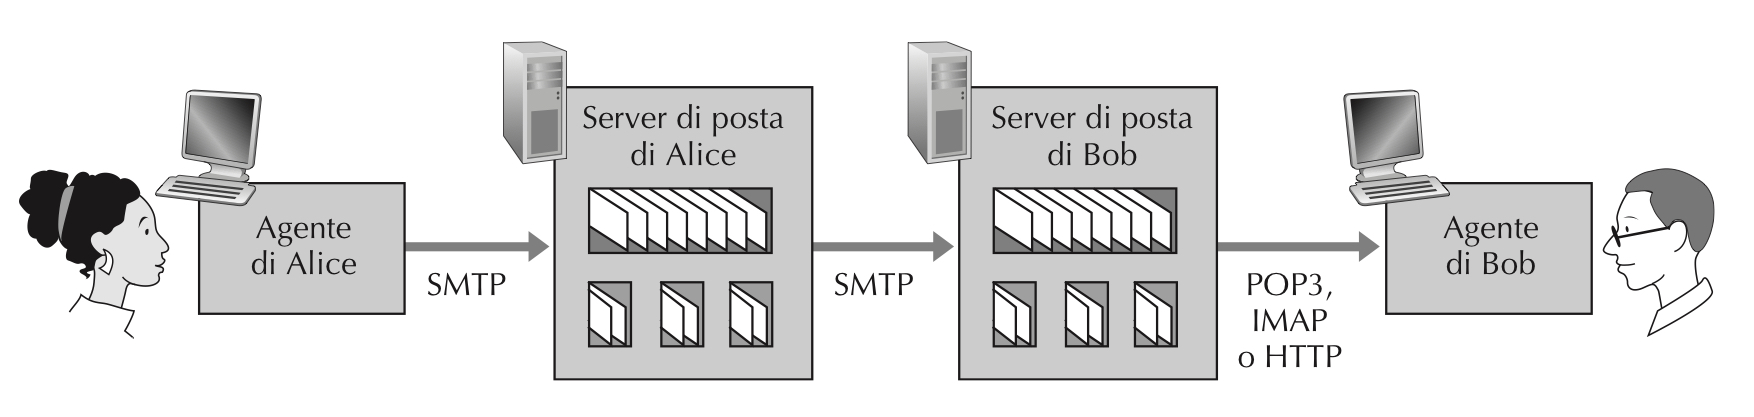
\includegraphics[width=12cm, height=20cm, keepaspectratio]{architettura_posta.jpg}
        \caption{Architettura della posta elettronica\cite{kurose2008reti}.}\label{architetturaPosta}
  \end{figure}


\subsection{Protocollo SMTP}
Il protocollo SMTP rappresenta il principale protocollo a livello applicativo per la posta elettronica. 
Fa uso del protocollo di trasporto TCP così da sfruttare il servizio di trasferimento dati affidabile. 
SMTP presenta un lato client e un lato server. Ogni server può eseguire entrambi i lati. 
Quando un server invia un messaggio di posta agisce come un client SMTP, mentre quando lo riceve si comporta 
da server SMTP.
SMTP trasferisce i messaggi di posta dal mail server del mittente al mail server del destinatario. 
Il protocollo SMTP di solito non utilizza mail server intermedi per inviare posta, anche quando i server finali 
sono collocati agli angoli opposti del mondo.
SMTP è un protocollo di tipo push, poiché la connessione TCP viene aperta dall’host che vuole inviare il messaggio. 
Il protocollo SMTP è simile ai protocolli umani utilizzati per la comunicazione. 
Prima di tutto il client SMTP apre una connessione TCP sulla porta 25 verso il server SMTP. 
Una volta stabilita la connessione client e server effettuano una sorta di presentazione prima di scambiarsi 
informazioni. Dopo la reciproca presentazione il client invia il messaggio.
Dato che SMTP utilizza connessioni persistenti, se un client ha più messaggi da inviare al server, 
può utilizzare la stessa connessione TCP per inviarli tutti. Una volta terminato di inviare tutti i messaggi, 
il client ordina a TCP di chiudere la connessione.
Di seguito un esempio di comunicazione SMTP:

\begin{verbatim}
    S: 220 smtp.example.com ESMTP Postfix
    C: HELO relay.example.com
    S: 250 smtp.example.com
    C: MAIL FROM: <bob@example.com>
    S: 250 OK
    C: RCPT TO: <alice@example.com>
    S: 250 OK
    C: DATA
    S: 354 End data with <CR><LF>.<CR><LF>
    C: From: "Bob" <bob@example.com>
    C: To: "Alice" <alice@example.com>
    C: Date: Tue, 15 January 2008 16:02:43 -0500
    C: Subject: Messaggio di prova
    C: 
    C: Ciao, questo è un messaggio di prova
    C: .
    S: 250 Ok: queued as 12345
        C: QUIT
    S: 221 Bye
\end{verbatim}\cite{SMTP}.

\subsection{Protocolli di accesso alla posta: POP3, IMAP, HTTP}
Come detto precedentemente SMTP è un protocollo di tipo push, utilizzato per l’invio di posta elettronica. 
Quindi l’user agent di un destinatario non potrà utilizzare questo protocollo per scaricare la posta dal suo mail 
server. Per compiere questa operazione è necessario utilizzare dei protocolli di tipo pull. 
Nei protocolli di tipo pull, la connessione TCP viene aperta da chi vuole ricevere i dati.
L’user agent di un destinatario di posta utilizzerà principalmente IMAP per scaricare la posta in locale dal suo mail server 
(POP3 ha delle limitazioni, quindi non è più molto utilizzato). 
Molte persone però accedono alla posta elettronica utilizzando il browser, in questo caso il protocollo utilizzato 
per scaricare i messaggi di posta è HTTP.

\subsection{Protocolli crittografici TLS/SSL}
SSL (secure sockets layer) permette di rendere sicuro TCP,  fornendogli servizi di sicurezza, 
comprese la riservatezza, l’integrità dei dati e l’autenticazione del server. 
Una versione particolare di SSL (SSLv3) è chiamata TLS (transport layer security).\cite{tls}

\begin{enumerate}
    \item \textbf{riservatezza}: il traffico viaggia cifrato;
    \item \textbf{integrità dei dati}: se non venisse assicurata l'integrità dei dati, un soggetto terzo
    potrebbe modificare il messaggio;
    \item \textbf{autenticazione da parte del server}: L'autenticazione TLS è unilaterale, solo il server si 
    autentica presso il client. Il mail client valida il certificato del server, controllando che la firma dei 
    certificati del server sia valida e riconosciuta da una certificate authority.
    In questo modo il mail client è sicuro dell'autenticità del mail server. 
    %Per questo motivo Postfix ha bisogno di un certificato da mostrare ai mail client.
\end{enumerate}


\subsection{Formato dei messaggi di posta elettronica}
Un messaggio di posta elettronica contiene una serie di righe di intestazione (header).
Ogni intestazione è una coppia chiave:valore. Alcune parole chiave sono opzionali (Subject:), 
ma altre sono obbligatorie come From: e To:. Una riga vuota separa gli header dal corpo del messaggio.
Di seguito un esempio di messaggio di posta:

\begin{verbatim}
    User-Agent: Microsoft-MacOutlook/16.49.21050901
    Date: Wed, 19 May 2021 12:12:08 +0200
    Subject: Importante
    From: Paolo Fagioli <paolo.fagioli@certimeter.it>
    To: Paolo Fagioli <palfag33@gmail.com>
    Message-ID: <9C8047BB-21D6-4D68-B33E-CCF3B68399DB@certimeter.it>
    Thread-Topic: Importante
    Mime-version: 1.0
    Content-type: text/plain;
        charset="UTF-8"
    Content-transfer-encoding: quoted-printable

    Invio un messaggio di prova.
    Saluti,

    Paolo Fagioli
\end{verbatim}